\documentclass{beamer-control}
\usepackage{beamer-control-singlefile}
\INCLUDEONLY{Reachability}
\begin{document}
\CONCEPT{Reachability}

\begin{SUMMARY}
\begin{itemize}
\item Reachability definition
\item Controllability definition
\item Reachability matrix
\item Reachable canonical form
\end{itemize}
\vfill References:
\begin{itemize}
\item \astrom{§7.1}
\end{itemize}
\end{SUMMARY}



\SUBCONCEPT{Definitions}

\begin{frame}{Reachability}
Consider a system where the state evolution is given by the linear state space equations
\[\frac{\mathrm{d} x}{\mathrm{d} t} = Ax+Bu\]
where $x$ is n-dimensional
\begin{itemize}
\item An important question is, is it possible to find a control signal $u(t)$ such that we can reach any state $x$ in the state space given an initial state $x_0$
\item The set of states that can be reached by steering the system with control input $u(t)$ for $0\leq t\leq T$ from an initial state $x_0$ is known as the \textit{reachable set}, $\mathcal{R}(x_0,\leq T)$
\end{itemize}
\end{frame}


\begin{frame}{Reachability}
\begin{itemize}
	\item A linear system is \textit{reachable} if,for any initial state $x_0$ and final state $x_f$, there exists a $T>0$ and control $u(t)$ such that $x(0)=x_0$ and $x(T)=x_f$
	\item In other words, the reachable set $\mathcal{R}(x_0,\leq T)$ is our whole state space
	\item This is essentially saying, we can get anywhere in our state space in finite time, no matter where we start!
\end{itemize}

\begin{figure}
	\centering
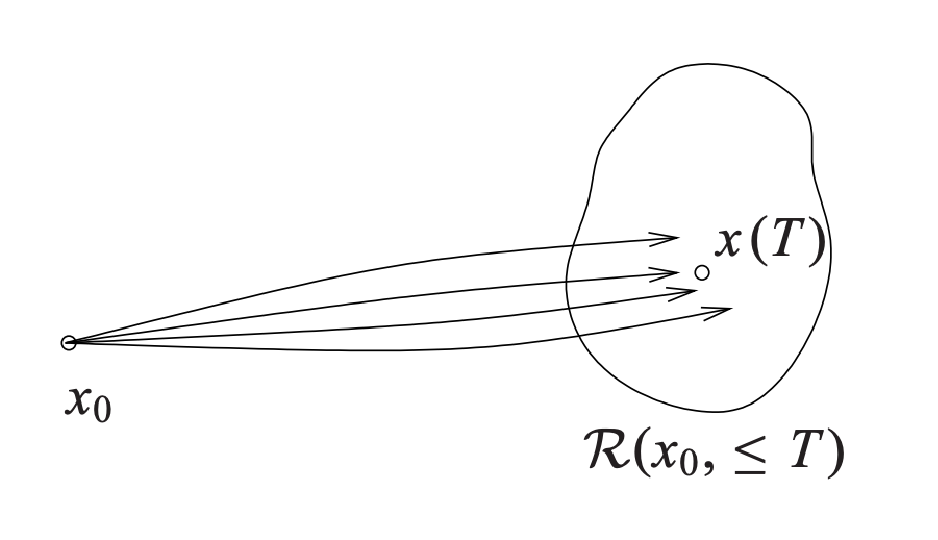
\includegraphics[width=0.5\linewidth]{figure7.1}
\\
\textbf{Figure 7.1:} The reachable set for a control system.
\end{figure}

\end{frame}	


\begin{frame}{Controllability}
	\begin{itemize}
		\item Reachability is related to a similar property called \textit{controllability}
		\item Rather than asking can we reach any state $x$ given an initial state $x_0$, controllability tackles the problem of controlling our system to a desired position $x_f$ based on a general starting position $x$
		\item These are subtly different but for linear systems, as we study in this course, reachability and controllability are equivalent
	\end{itemize}
\end{frame}


\SUBCONCEPT{Tests for reachability}

\begin{frame}{Reachability matrix}
	\begin{itemize}
		\item Define the reachability matrix
		\[W_r = \begin{bmatrix}
			B & AB & A^2 B & \cdots & A^{n-1}
		\end{bmatrix}\]
		\item A linear system is reachable if and only if the reachability matrix $W_r$ is invertible (or equivalently, full rank)
	\end{itemize}

\end{frame}

\begin{frame}{Example}
	Consider the simplified balance system (which is a model for many examples which the centre of mass is above a pivot point i.e. segway, inverted pendulum)
	\begin{align*}
		(M+m)\ddot{p}-ml\cos \theta \ddot{\theta} &= -ml\sin\theta \dot{\theta}^2+F,\\
		(J_ml^2)\ddot{\theta} -ml\cos \theta \ddot{p} &= mgl\sin \theta.
	\end{align*}
	Linearising around $(p,0,0,0)$ gives us the state space matrices
	\[ A=\begin{bmatrix}
		0 & 0 & 1 & 0\\
		0 & 0 & 0 & 1\\
		0 & m^2l^2g/\mu & 0 & 0 \\ 0& M_tmgl/\mu & 0 & 0
	\end{bmatrix}, \quad
	B = \begin{bmatrix}
		0 \\ 0 \\ Jt/\mu \\ lm/\mu
	\end{bmatrix}\]
	where $\mu=M_tJ_t-m^2l^2$, $M_t=M+m$, and $J_t=J+ml^2$
\end{frame}

\begin{frame}{Example continued}
The reachability matrix is
\begin{align*}
	W_r&= \begin{bmatrix}
		B & AB & A^2 B & A^3B
	\end{bmatrix} \\ 
	W_r &= \begin{bmatrix}
		0 & J_t/\mu & 0 & gl^3m^3/\mu^2 \\ 
		0 & lm/\mu & 0 & gl^2m^2M_t/\mu^2 \\
		J_t/\mu & 0 & gl^3m^3/\mu^2 & 0 \\
		lm/\mu & 0 & g^2l^2m^2M_t/\mu^2 & 0 
	\end{bmatrix}
\end{align*}
The determinant of this matrix is $\operatorname{det}(W_r)=-\frac{g^2l^4m^4}{\mu^6}(MJ+mJ+Mml^2)^2\neq 0$ and therefore, the reachability matrix is invertible and so the balance system is reachable!
\end{frame}

\SUBCONCEPT{Reachable canonical form}

\begin{frame}{Coordinate transformation}
\begin{itemize}
	\item Changing the coordinates and writing dynamics in this transformed coordinate system $z=Tx$ often makes calculation more convient
	\item Reachable canonical form is given by 
	\[\frac{\mathrm{d}z}{\mathrm{d}t} = \begin{bmatrix}
		-a_1 & -a_2 & -a_3 &  \cdots & -a_n	\\
		1 & 0 & & & \\
		& 1& 0 & & & \\
		& & \ddots & \ddots  & \\
		& & & 1 & 0
			\end{bmatrix}z + \begin{bmatrix}
			1 \\ 0 \\ 0 \\ \vdots \\ 0
			\end{bmatrix} u \]
			\[y=\begin{bmatrix}
				b_1 & b_2 & b_3 & \cdots & b_n
			\end{bmatrix}z + du\]
\end{itemize}
\end{frame}

\begin{frame}{Coordinate transformation}
\begin{itemize}
	\item The characteristic polynomial for a system in reachable canonical form is 
	\[\operatorname{det}(sI-A)= s^n+a_1s^{n-1}+\cdots + a_{n-1}s+a_n\]
	\item The reachability matrix in reachable canonical form is
	\[\tilde{W}_r = \begin{bmatrix}
		1 & -a_1 & a_1^2-a_2 & & \\
		0 & 1 & -a_1 & & * \\
		& & \ddots & \ddots & \\
		&  & & 1 & -a_1 \\
		& & & & 1
	\end{bmatrix}\]
	where $*$ are possible nonzero terms
	\item The transformation matrix $T$ can be found by 
	\[T=\tilde{W_r} W_r^{-1}\]
\end{itemize}
\end{frame}


\SUMMARYFRAME
\FINALE

\end{document}
